\documentclass{cmspaper}
\usepackage{graphicx}
\begin{document}

%==============================================================================
% title page for few authors

\begin{titlepage}

% select one of the following and type in the proper number:
%   \cmsnote{2008/000}
  \internalnote{2008/000}
%  \conferencereport{2005/000}
   \date{6. October 2008}

  \title{A Cross-Cleaning Package}

  \begin{Authlist}
    Christian~Autermann, Benedikt~Mura, Friederike~Nowak
       \Instfoot{uhh}{Universit\"at Hamburg, Germany}
    Jean-Roch~Vlimant
       \Instfoot{ucsb}{University of California, Santa Barbara, USA}

    %%@@ Anyone else ???

  \end{Authlist}

% if needed, use the following:
%\collaboration{Flying Saucers Investigation Group}
%\collaboration{CMS collaboration}

%  \Anotfoot{a}{On leave from prison}
%  \Anotfoot{b}{Now at the Moon}

  \begin{abstract}
    The reconstructed objects like electrons, photons, muons, taus, and
    jets may have an overlap in energy, i.e. at least one shared and therefore
    double counted energy cell. This note discusses the cross-cleaning package
    which provides algorithms to identify the overlap of any two objects. The
    package provides a framework to consistently correct objects, or to remove
    doublicates. 
    %%@@ Is this really true, i.e. does it work with RECO objects?
    The cross-cleaning package is designed to run on {\sc Reco} objects before
    {\sc Pat}-tification but can be run for development and debugging on {\sc
    Pat} objects, too.
  \end{abstract} 

% if needed, use the following:
%\conference{Presented at {\it Physics Rumours}, Coconut Island, April 1, 2005}
%\submitted{Submitted to {\it Physics Rumours}}
%\note{Preliminary version}
  
\end{titlepage}

\setcounter{page}{2}%JPP


\section{Introduction}
The multiple counting of any energy fraction must be
avoided in order to obtain optimal energy resolutions of these objects. This is
especially true for the missing transverse energy (MET). The details how the
shared energy is split between two objects will depend on the details of each
analysis. In this note a cross-cleaning package~\cite{package} is discussed,
that is flexible enough to allow the implementation any energy splitting
algorithm between objects. If more than two objects share energy, circular
dependencies may arise. These possible interferences are dealed with, so that
the outcome of cross-cleaned objects does not depend on the order in which the
cleaning algorithms are called.


\section{The Cross-Cleaning-Algorithm Framework}
The cross-cleaning is performed in two steps: First binary cleaners, i.e.
specialized algorithms that clean two collections of objects against eachother,
are called (for example electron-vs.-photon cleaner, muon-vs.-jet cleaner etc.).
These binary cleaners do not apply any corrections on either of the two input
collections, but save the result of the cleaning algorithms in an internal map.
An entry in this map would be the object that should be corrected, the object
that is causing this correction, and finally the information how the object
should be corrected. This scheme is illustrated in Fig.~\ref{fig:Cleaning}.

\begin{figure}[hbtp]
  \begin{center}
    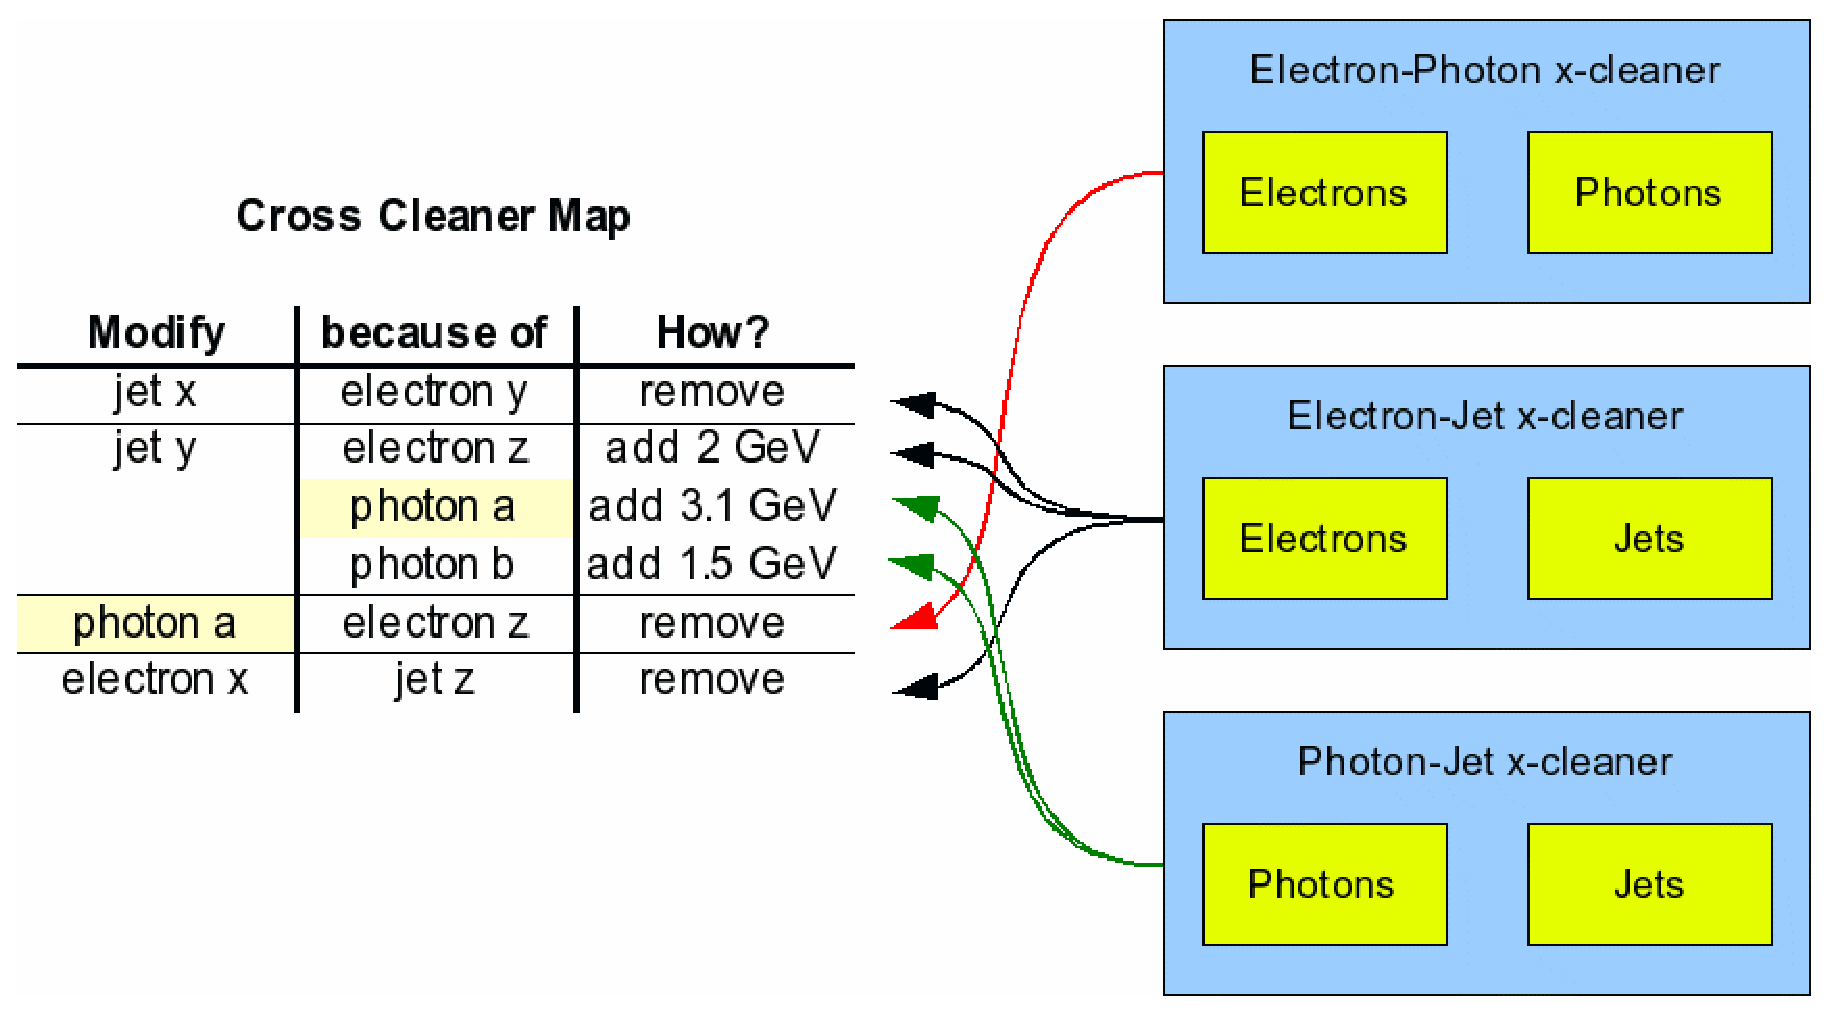
\includegraphics[scale=.4]{CleaningMap.eps}
    \caption{This figure illustrates the input and the result of different
    cleaning algorithms. Each algorithm takes two collections of any objects,
    and creates an entry in the internal cross-cleaning map for each object that
    should be modified.}
    \label{fig:Cleaning}
  \end{center}
\end{figure}

In a second step, this temporary buffer map is scanned for possible conflicts.
If the same object {\it A} is causing a correction to object {\it B} but should
be corrected itself because of object {\it C}, than it might happen that after
the correction of {\it A} the correction of {\it B} is no longer necessary or at
least different to the case where first {\it B} is corrected and then {\it A}.
The result of the cross-cleaning must not depend on the order in which objects
are compared, therefore conflicts are resolved before any object is
modified.

%%@@ This needs to be revised
Possible conflicts can be resolved since all decisions of the cleaning
algorithms are saved in the internal map and not yet applied on the objects. The
order of the foreseen corrections can be changed, or single corrections may be
revised. Again, the details how these decisions are made, may depend on the
specific analysis. 
%%If I understand the implemented algorithm correctly, than the following is
%%happening:
%% A to be dropped because of C
%%  ...
%% C to be dropped because of X
%% Where A,B,C.. refer to the position in the map.
%% Then the last action (dropping of C) is not performed.
%%
%% -> In case of conflicts the position in the map defines which object is
%% removed, do I understand this correctly?
%% -> Shouldn't we had a case differentiation wether A or C is dropped, lets say
%% by pT?
%
%%Proposal:
By default, from the set of map-entries that are in conflict with eachother,
that entry is removed from the map, whose object causing that entry is smallest
in $p_T$. For each set of map-entries this step is repeated, until all conflicts
are resolved.

After the objects have been cross-cleaned, the properties of these objects have
to be recalculated. All properties related to the energy deposition in the
calorimeter or the cross-cleaning objects, may have changed. Isolation
algorithms, energy scale correction algorithms, etc. have to be re-run.

The raw MET is calulated from calorimeter towers only and will not be changed by
this cross-cleaning. However, the missing $E_T$ correction can either be
recalculated using the new collections of corrected objects as input, or by
tracking the impact of each cross-cleaning modification on the MET. This
package~\cite{package} provides a corrected MET object using the latter way.
Both ways should give the same result and the comparison is a valuable
cross-check. 

The cross-cleaning package is a producer, that creates new collections of
(cross-cleaned) objects. If for a specific event no cross-cleaning was done,
then these ouput collections are equal to the input collections. Additionally,
collections of dropped objects are created, i.e. if one object was dublicated
(for example an electron, that was a jet, too) than either object was dropped
and written into a ``dropped'' collection, while the other object remains in the
normal output collection. 
%%@@ Does the following already work?
For debugging purpose a reference map can be written into the event, that
associates every input object with the ouput object which can be either in the
normal output collection or in the ``dropped'' collection.

\section{Electron - Photon Cleaner}
\subsection{Algorithm}
\subsection{Validation}

\section{Electron - Jet Cleaner}%%Or better: EM-object - jet Cleaner ???
%% \section{Photon - Jet Cleaner}
\subsection{Algorithm}
\subsection{Validation}

\section{Muon - Jet Cleaner}
\subsection{Algorithm}
\subsection{Validation}

\section{Conclusion}


\pagebreak
\begin{thebibliography}{9}
  \bibitem {package} {\bf The CVS code repository},
    \underline{http://cmssw.cvs.cern.ch/cgi-bin/cmssw.cgi/UserCode/SusyAnalysis/PatCrossCleaner/}

  \bibitem {twiki} {\bf The online documentation},
    \underline{https://twiki.cern.ch/twiki/bin/view/CMS/SusyPatCrossCleaner/}

  \bibitem {met} {\bf The online documentation},
    \underline{https://twiki.cern.ch/twiki/bin/view/CMS/SusyPatCrossCleaner/}

\end{thebibliography}
 
%------------------------------------------------------------------------------

\end{document}
